%%%%%%%%%%%%%%%%%%%%%%%%%%%%%%%%%%%%%%%%%%%%%%%%%%%%%%%%%%%%%%%%%%%%%%%%%%%%%%%%
%	TRABAJO: Proyecto Integrador
%		Titulo: 	Desarrollo de IP cores con procesamiento de Redes de Petri 	
%					Temporales para sistemas multicore en FPGA					
%		Autores:	Juli�n Nonino												%					Carlos Renzo Pisetta										%		Director:	Orlando Micolini											
%%%%%%%%%%%%%%%%%%%%%%%%%%%%%%%%%%%%%%%%%%%%%%%%%%%%%%%%%%%%%%%%%%%%%%%%%%%%%%%%

% Path im�genes: ./resultado_conclusiones/resultados/img
% Nombre predeterminado im�genes: resultadosxx
%	xx es el numero de imagen

\section{Problema: \emph{F�brica de Mesas}}
	\label{sec:problema_fabrica_mesas}
		
	El problema de la f�brica de mesas, ha sido inventado para �ste trabajo con el objetivo de verificar el funcionamiento del procesador de Redes de Petri Temporizadas, como se vi� en la secci�n \ref{sec:fabrica_mesas}, p�gina \pageref{sec:fabrica_mesas}.
	
	La idea fundamentalmente es crear una l�nea de producci�n donde en cada etapa existan repositorios de recursos (\emph{variables}) y trabajadores (\emph{hilos/procesos}) accedan a ellos, realicen un procesamiento  sobre los mismos con una determinada duraci�n.
	
	\newpage
		
	\subsection{Modelo del problema}
			
		Modelando el problema, se obtiene la siguiente Red de Petri (Figura \ref{fig:resultados35}).
		\begin{figure}[H]
			\centering
			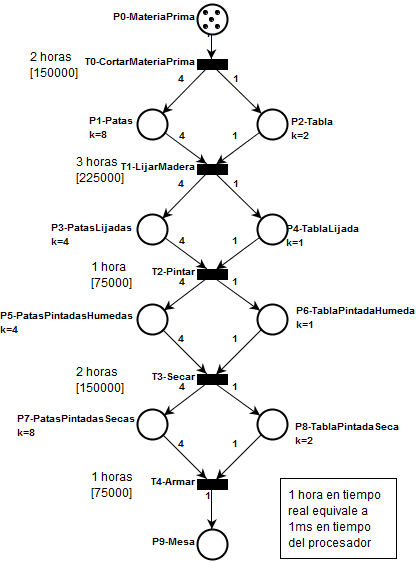
\includegraphics[width=0.9\linewidth,keepaspectratio]{./resultados_conclusiones/resultados/img/resultados35}
			\caption{Red de Petri que modela el problema de la f�brica de mesas}
			\label{fig:resultados35}
		\end{figure}
	
	\newpage
			
	\subsection{Mediciones realizadas}
		
		Utilizando los c�digos fuentes incluidos en el ap�ndice \ref{ap:codigos_programas}, para la ejecuci�n con sem�foros el mostrado en la secci�n \ref{sec:programa_fabrica_mesas_sem} de la p�gina \pageref{sec:programa_fabrica_mesas_sem}, y, para la ejecuci�n con Redes de Petri el c�digo de la secci�n \ref{sec:programa_fabrica_mesas_petri} de la p�gina \pageref{sec:programa_fabrica_mesas_petri}.
		
		\begin{figure}[H]
			\centering
			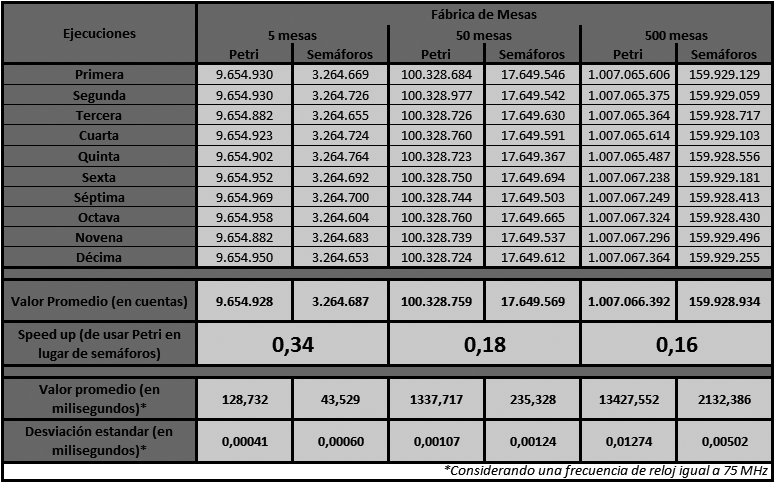
\includegraphics[width=1\linewidth,keepaspectratio]{./resultados_conclusiones/resultados/img/resultados36}
			\caption{Tabla de mediciones realizadas para el problema de la f�brica de mesas}
			\label{fig:resultados36}
		\end{figure}
			
	\subsection{An�lisis de los resultados obtenidos}
	
		La imagen anterior, muestra que el procesador de Redes de Petri tiene un peor desempe�o que la resoluci�n con sem�foros. �sto, se debe a que la resoluci�n con Redes de Petri utiliza interrupciones, lo que implica que se debe suspender al hilo mientras espera que su disparo sea realizado. El problema es que, con el sistema operativo utilizado (Xilkernel), la �nica manera de suspender un hilo y quitarlo de la planificaci�n de procesos es utilizar sem�foros. Por �sta raz�n, no es posible hacer una comparaci�n adecuada entre el procesador de Redes de Petri y la resoluci�n utilizando sem�foros debido a que el programa que utiliza el procesador de Redes de Petri tambi�n debe utilizar sem�foros.
		
		Adem�s, cada interrupci�n que se produce implica que se cambie de contexto hacia el proceso encargado de atender la interrupci�n y luego, se vuelva a darle el control a los hilos del sistema. �sto tambi�n genera que el valor de tiempo medido al resolver el problema con el procesador de Redes de Petri aumente.
		